\chapter{Domain split approach: application to k-medoids problem}
\label{chap:prior_split}
%\textit{In this chapter are presented Prior works leading to \af. In Section~\ref{sec:relaxation} we explain how to tackle \csps{} by modeling it through a continuous optimization problem, as a first attempt aiming for the right direction in order to find the proper approach. In Section~\ref{sec:split} we present a brief work where we applied the the {\it problem subdivision} approach to solve the {\it k-medoids problem} in parallel. Finally we present in Section~\ref{sec:paramils} a study applying the {\sc ParamILS} tool in order to find the optimum parameter configuration to {\it Adaptive Search} solver.}
\textit{In this appendix a prior works leading to \posl{} is presented: a brief work where we applied the {\it problem subdivision} approach to solve the {\it k-medoids problem} in parallel, as a first attempt aiming for the right direction in order to find the proper approach.} 

\vspace{2ex}\vfill
\minitoc
\newpage

\section{Introduction}

Usually, to solve some problems using parallelism, our first thought is either partitioning the problem into a set of sub-problems, or dividing its search space. In both cases, the idea is to solve a set of problems, all of them smaller and easer than the original one, and combining all solutions to obtain the solution of the original problem. In \cite{Arbelaez2012} \etal{Arbelaez} present a study of the impact of space-partitioning techniques on the performance of parallel local search algorithms to tackle the \textit{k-medoids} clustering problem. Authors use a parallel local search, in order to improve the scalability of the sequential algorithm, which is measured, in terms of the quality of the solution, with respect to the sequential algorithm. In this work two main techniques for domain partitioning are presented: {\it space-filling curves}, used to reduce any n-dimensional representation into a one-dimension space; and {\it k-Means} algorithm. We found that the used methods for domain partitioning do not take into account the number of clients associated to each new sub-domain. This results in an unbalanced distributions of workload phenomenon. For that reason the goal of this study was designing some ideas to tackle the same problem. \footnote{This work falls within the framework of the Ulysses project between France and Ireland.}

The \textit{k-medoids} problem aims to select a subset $M$ of $k$ points (the medoids) from a set of points $S$, such that the average distance from any point to its closest medoid is minimized. It finds a lot of applications in the industry, like in resource allocation, data mining, among others. It is quite similar to \textit{k-means} problem, except that the set of medoids $M$ is forced to be a subset of $S$.

Algorithm~\ref{algo} represents the backbone of our idea. This algorithm takes a set of $\mathbb{R}^2$ {\it points} (representing the locations of the clients) and returns a partition of size $K$. Such a set of points is called a {\it domain} and the partition a {\it sub-domain}. At each intermediate step $i$, we have a set (list) of sub-domains. The algorithm takes the most populated one, splits it into two (or four, depending on the strategy) new sub-domains and includes them in the list. The stop condition will depends on the fallowed approach (see below).

\incmargin{1.4em}
\linesnumbered
\begin{algorithm}[H]
\dontprintsemicolon
\SetLine
\SetKwData{A}{A}
\SetKwData{Q}{Q}
\SetKwData{Uni}{U}
\SetKwData{subsets}{$\left[a_1, a_2\right]$}
\SetKwData{suba}{$a_1$}
\SetKwData{subb}{$a_2$}
\SetKwFunction{GetNext}{GetNext}
\SetKwFunction{Split}{Split}
\SetKwFunction{Insert}{Insert}
\SetKwInOut{Input}{input}
\SetKwInOut{Output}{output}

\Input{\Uni : Set of client locations}
\Output{\Q = $\left\{Q_i\right\}_{i=1\dots K}$: $K$ subsets of \Uni}
\BlankLine

\A $\leftarrow$ \Uni\;
\Q .\Insert{\A}\;
\Repeat{$<$some condition$>$}{ \nllabel{paso_condicion} 
	\A $\leftarrow$ \Q .\GetNext{} \label{paso2} \tcc{It also removes the returned element}
    \subsets $\leftarrow$ \Split{\A} \label{paso3}\;
    \Q .\Insert{\suba , \subb} \label{paso4}\;
}
\caption{Domain\_Split}
\label{algo}
\end{algorithm}

First of all, we make clear some details of the algorithm presented above:

\begin{itemize}
\item \texttt{Insert($\dots$)} Inserts a set (or two) into the data structure. % \footnote{The design was decided, because first we need to know some implementations details about the tool already coded by the Ireland team}.
\item \texttt{GetNext()} Returns the next sub-set to be divided, tacking into account the {\it split strategy} (see below).
\item \texttt{Split($\dots$)} Returns two sub-domains as a subdivision of the given domain (parameter).
\end{itemize}

In the next sections we answer two main question arising at this point:

\begin{enumerate}
\item \textit{How to split the each sub-domain?} ($<$\emph{Split}$>$ function on line \ref{paso3}) It refers to, given a set of points (locations), how to decide which of them will be included into one sub-domain and which of them into the other.
\item \textit{How much to split each sub-domain?} ($<$\emph{some condition}$>$ on line \ref{paso_condicion}) It refers to deciding when to stop splitting the domain.
\end{enumerate}

\section{Domain Splitting. General point of view}

In order to split the domain, we can think in some approaches, taking into account the number of available cores and the number of metro-nodes we want to place in the system. In the article of A.~Arbelaez and L.~Quesada a domain split taking into account the number of available cores for parallel calculus is proposed. In our approach we intend to extend this idea keeping in mind also the number of metro-nodes to allocate. Following, we propose three variants to face the problem:

% itemize variants, give the main idea in 1 or 2 paragraphs for each variant.

\begin{enumerate}
\item {\bf one metro-node per core}: In this variant we can assign one metro-node to each core, and in this case, splitting the domain in $K$ sub-domains ($K$ is the number of cores). It means that the algorithm will compute the best position for a metro-node in a current sub-domain. \label{var1}
\begin{itemize}
\item In this case we only have to replace the line \ref{paso_condicion} by something like:  \textcolor{gray}{{\bf for} $i \leftarrow 1$ {\bf to} $N$ {\bf do} $\dots$}, 
where $N$ is the number of metro-nodes.
\item The ideal scenario here is when $N = K$ which is not probable at all. So we only should study the case when they are different
\item In that case, we need to distribute efficiently the metro-nodes into the domain subdivisions, but here, one possible scenario arise: depending on the followed domain-split strategy, we can be trying to allocate a metro-node into an area with a few clients. This produces a very local point of view of the problem. That is the reason why the following \textit{second variant} is proposed.
\end{itemize}
\item {\bf Incomplete partition}: To split a sub-domain if it can generate sub-sub-domains containing at least $C$ clients. It means, for example, if there exist in the list a sub-domain with 8 clients, and the number $C$ is fixed in $C = 5$, this sub-domain can not be divided, because it will generate for sure a sub-sub-domain with less that 5 clients. In this case more than one metro-node would be allocated in some of those specific sub-domains, because we can have more metro-nodes than sub-domains in our model. Of course, using this variant we can find situations described in the first variant. In that case we should proceed consequently. \label{var2}
%\begin{itemize}
%\item Of course, using this variant we can find situations described in the first variant. In that case we should proceed consequently.
%\end{itemize}
\item {\bf Combination}: This variant is just a combination of the two previous variants. Then, two parameters have to be tuned: \label{var3}
\begin{itemize}
\item $C \rightarrow$ Lower bound of clients for new sub-domains, i.e. a sub-domain can be divided iff the new produced sub-domains will contains more than $C$ clients.
\item $M \rightarrow$ Lower bound of metro-nodes to be allocated in a sub-domain. In this case the domain is split while it can be ensure that at least $M$ metro-nodes will be assigned to each sub-domain.
\end{itemize}
\end{enumerate}

% itemize split startegies, give the main idea in 1 or 2 paragraphs for each.

\section{Split strategies}

In this section three ideas to split the domain are discussed. They take a sub-domain and produce other two, dividing the space vertically or horizontally, depending on the shape of the current sub--domain. In other section I expose another strategy to follow, in which the subdivision of a sub-domain produces four sub-domains. In all of them, the number of clients in each sub-domain is taken into account, but in different ways. A common feature between them is that they split a given sub-domain perpendicularly (either to the x--axis or to the y--axis, depending on the characteristic of the sub-domain to be divided). The reference point to divide the sub-domain is called the {\it cut point} of the sub-domain.

\begin{figure}
	\centering
	\subfloat[][Geometrical Split]{%
		\label{norm:geom}
		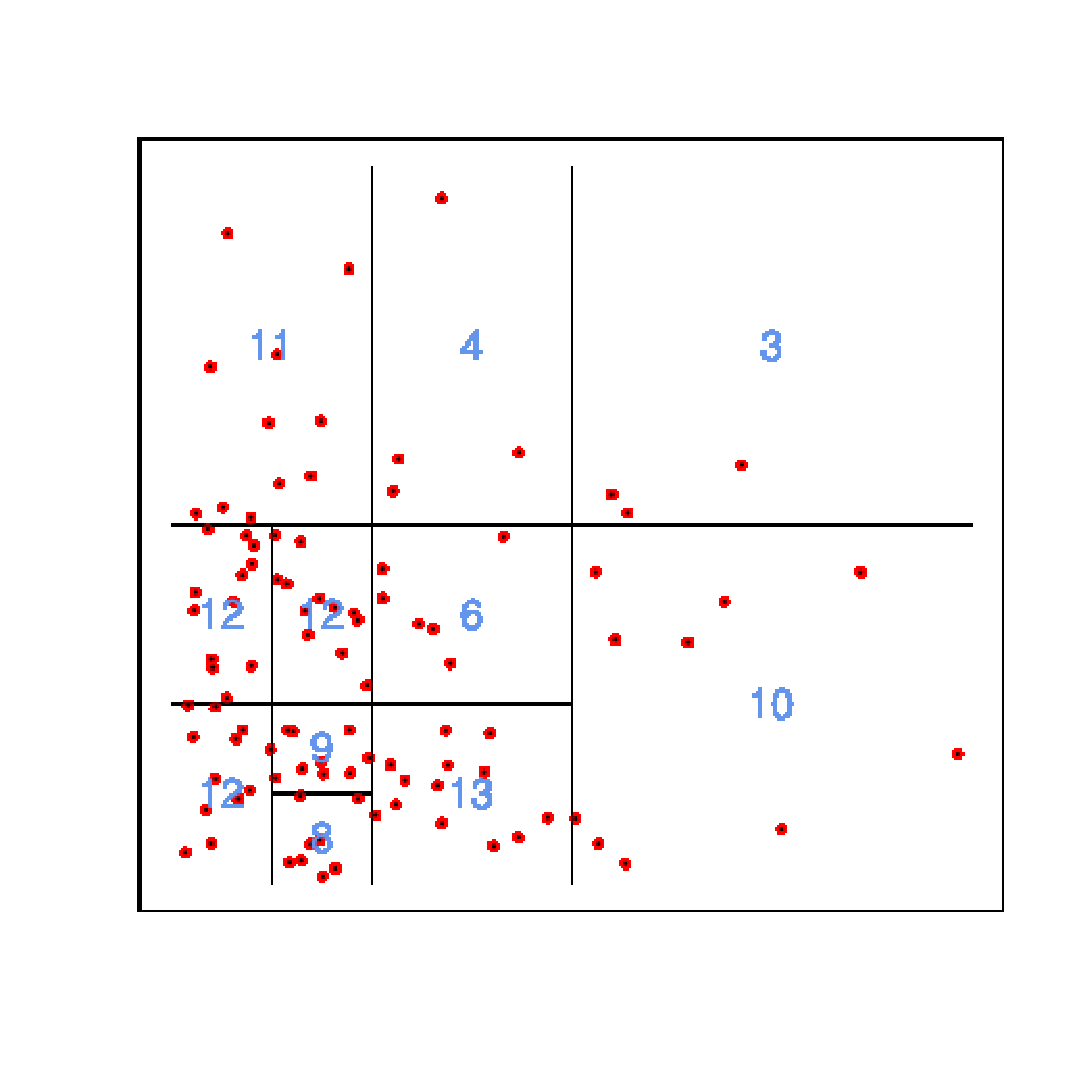
\includegraphics[width=0.3\textwidth]{norm_geom.eps}
	}
	\hspace{3pt}%
	\subfloat[][Cardinal Split]{%
		\label{norm:card}%
		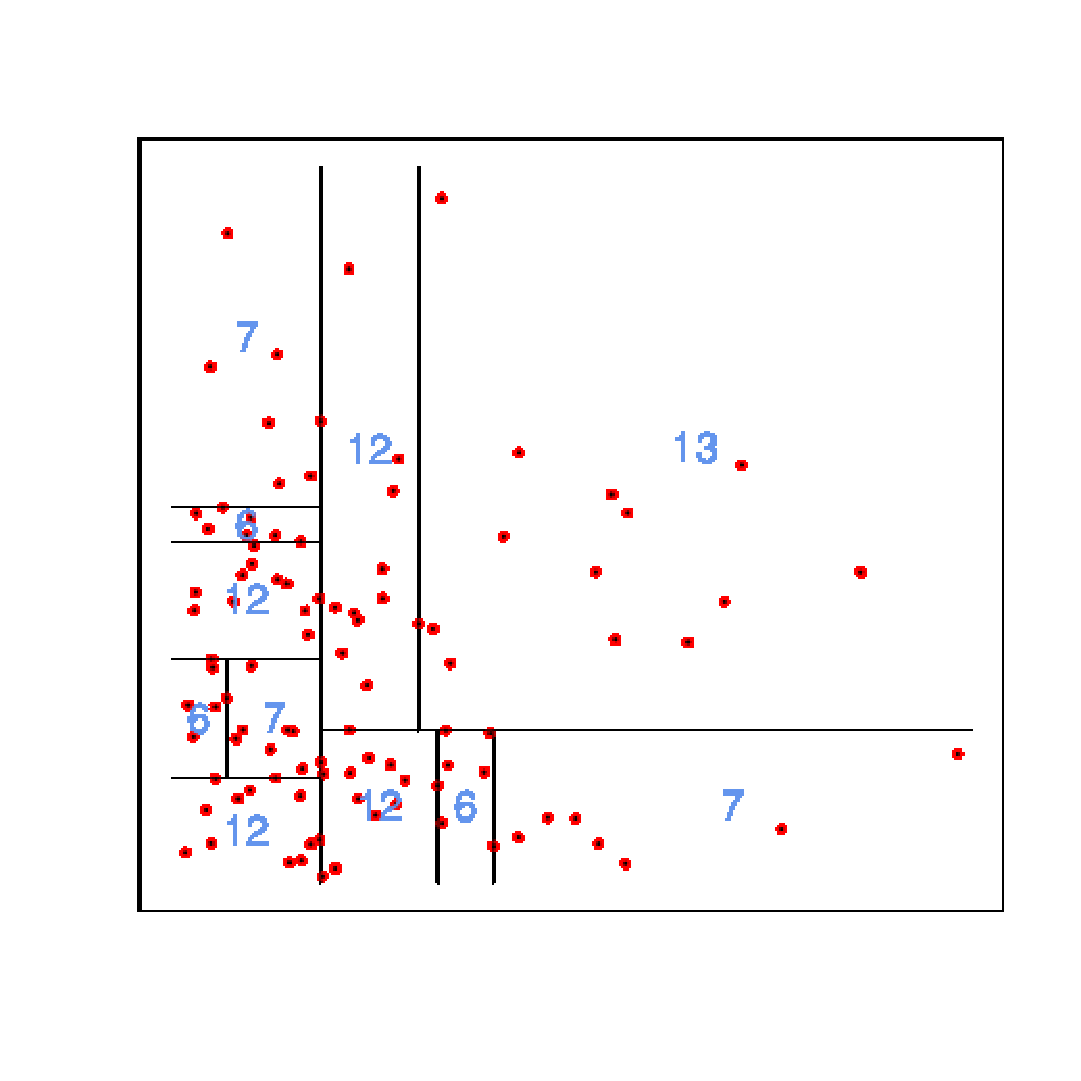
\includegraphics[width=0.3\textwidth]{norm_card.eps}
	}
	\hspace{3pt}%
	\subfloat[][Mean Split]{%
		\label{norm:mean}%
		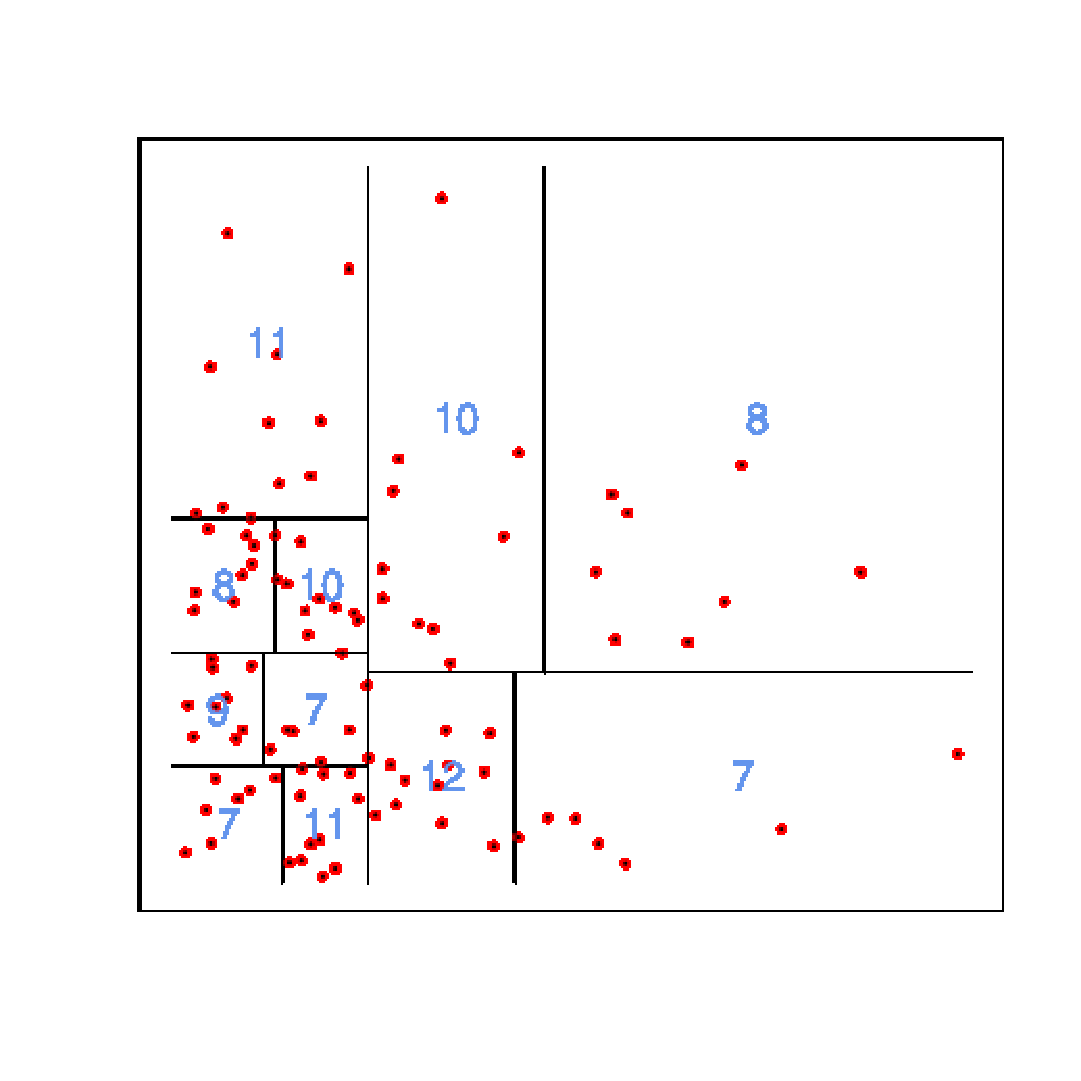
\includegraphics[width=0.3\textwidth]{norm_mean.eps}
	}
	\caption[]{Split domain of point normally distributed $\mathcal{N}\left(0,0.35\right)$}%
	\label{split:norm}
\end{figure}

\begin{figure}
	\centering
	\subfloat[][Geometrical Split]{
		\label{unif:geom}
		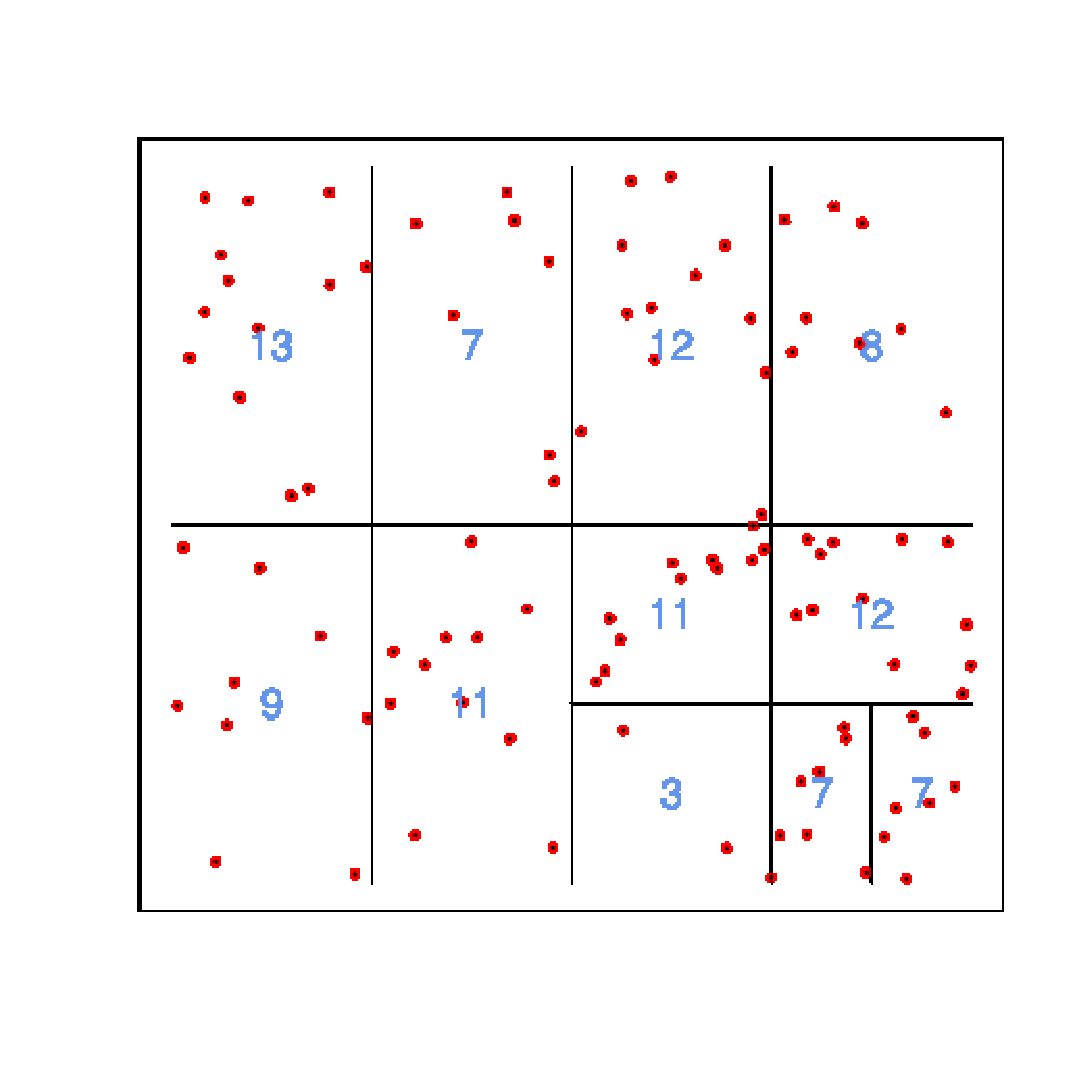
\includegraphics[width=0.3\textwidth]{unif_geom.eps}
	}
	\hspace{3pt}%
	\subfloat[][Cardinal Split]{%
		\label{unif:card}%
		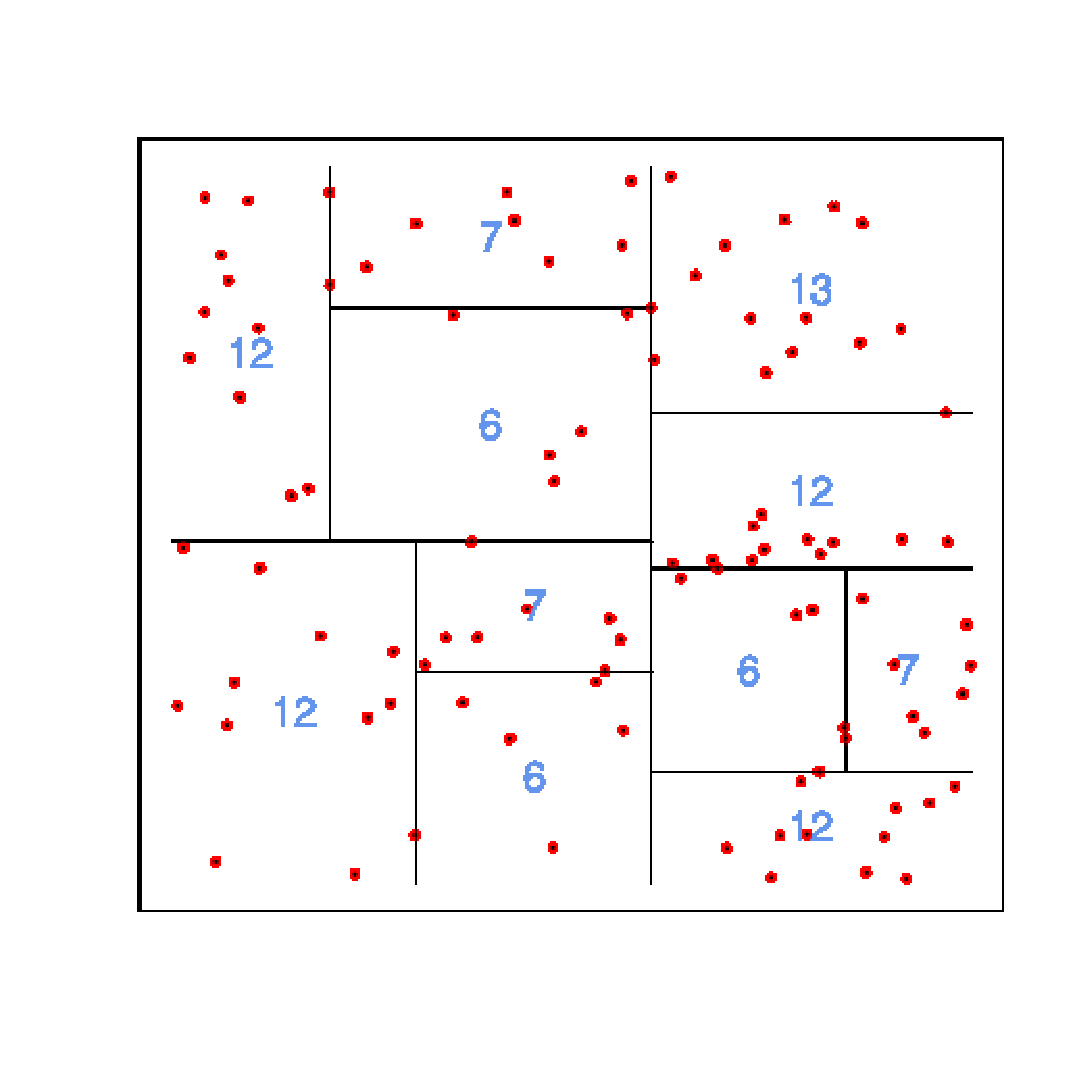
\includegraphics[width=0.3\textwidth]{unif_card.eps}
	}
	\hspace{3pt}%
	\subfloat[][Mean Split]{%
		\label{unif:mean}%
		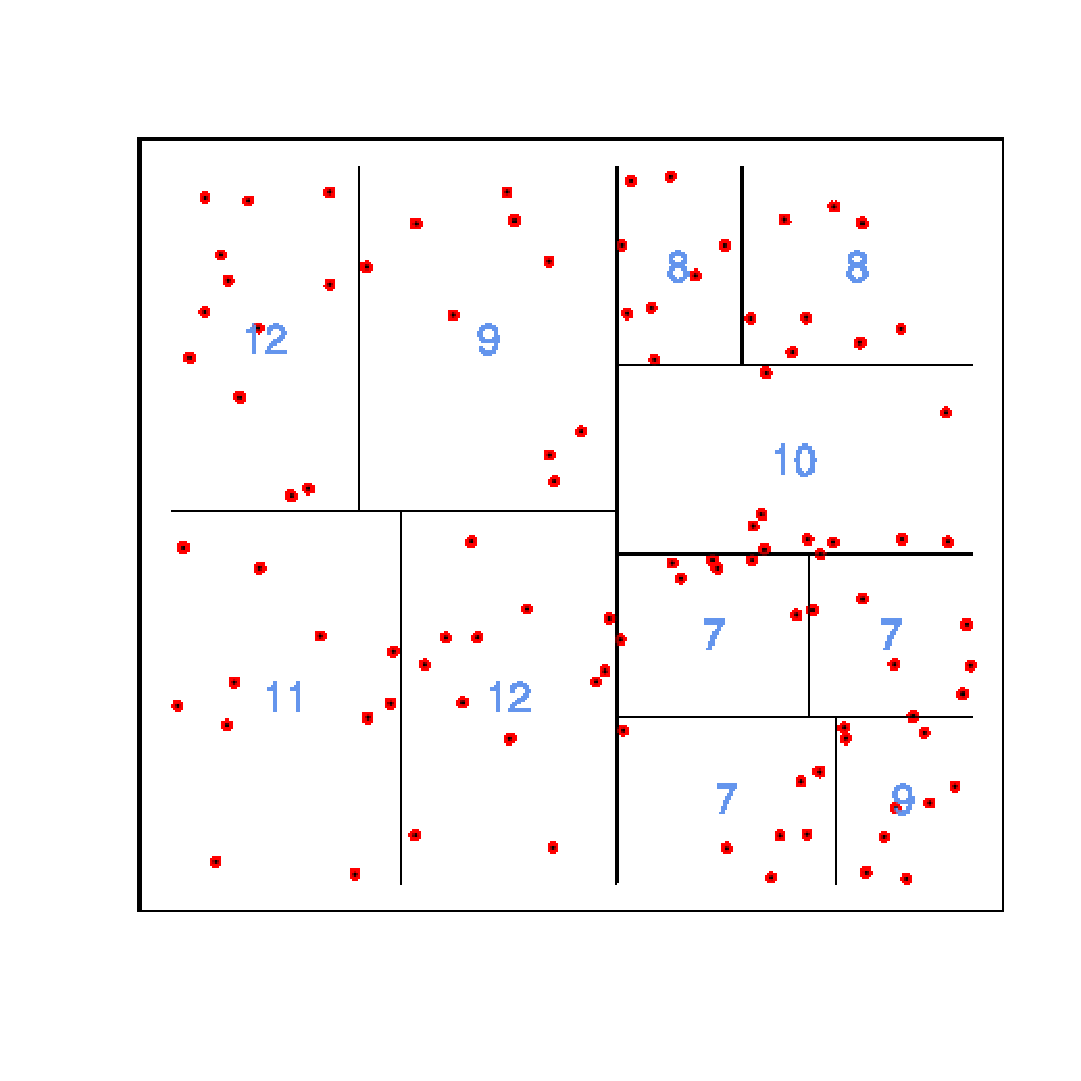
\includegraphics[width=0.3\textwidth]{unif_mean.eps}
	}
	\caption[]{Split domain of point uniformly distributed}%
	\label{split:unif}
\end{figure}

\begin{figure}
	\centering
	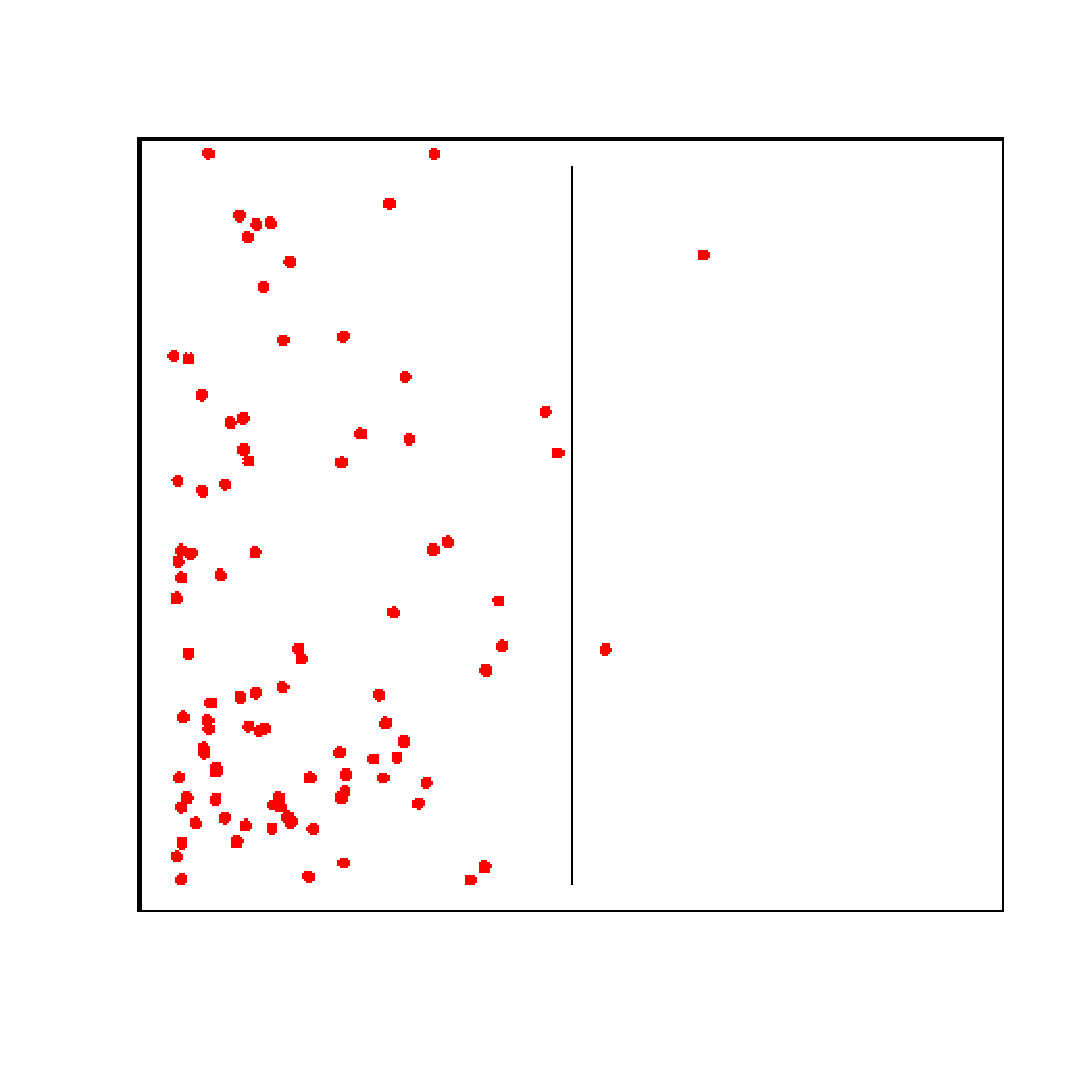
\includegraphics[width=0.3\textwidth]{badGeo.eps}
	\caption[]{If we assume $C = 3$ then this set can't be divided}%
	\label{fig:badGeom}
\end{figure}

\begin{enumerate}
\item {\bf Geometrical Split}: 
\begin{itemize}
\item \underline{Split criterion}: {\it Geometrical} $\rightarrow$ Dividing the region in tow parts with the same area.
\item \underline{Cut point}: The middle point of the x--axis (or y--axis, depending on the shape)
\item \underline{Result}: Two equal regions, but with different amount of clients (see Figure~\ref{norm:geom}). In the next step, the next sub-domain to divide will be, from those already divided, the most populated one (the sub-domain with more clients).
\item \underline{Problem}: Sometimes a sub-domain must be divided because it has a lot of client, but in the other hand it generates a sub-domain with a few clients, as we can see in the Figure~\ref{fig:badGeom}.
\item \underline{Benefit}: Very fast split. If we attack scenarios with point uniformly distributed, the behavior is pretty much desirable, as we can see in the Figure ~\ref{unif:geom}. 
\end{itemize}

\item {\bf Cardinal Split}
\begin{itemize}
\item \underline{Split criterion}: The number of clients, i.e., a sub-domain is divided in such a way that in the resulting sub-sub-domains there are the same number of clients.
\item \underline{Cut point}: The current sub-domain is ordered and the x--axis (or y--axis, depending on the shape) of the element (location of the client) right in the center is selected to be the {\it cut point}
\item \underline{Result}: Two regions with the same ($\pm 1$) amount of clients (see Figure~\ref{norm:geom}). In the next step, the next sub-domain to divide is, from those already divided, the most populated one (the sub-domain with more clients).
\item \underline{Problem}: The subdivision process is a bit more costly: we need to group the clients on both sides of a {\it perfect pivot}\footnote{Element of a set with the same number of elements lower and greater than him}.
\item \underline{Benefit}: It guarantees the same cardinality in both new sub-sub-domains.
\end{itemize}

\item {\bf Mean Split}
\begin{itemize}
\item \underline{Split criterion}: This is a mid-point strategy between the two previous. The goal is to find a {\it cut point} to group the elements of the current sub-domain, but in a easy way (fast), for that reason we do not compute the exact middle point to produce two sub-sub-domains with the same cardinality, as in the previous approach, instead of that we work with his expected value: the arithmetic mean.
\item \underline{Cut point}: The mean of the $x$--axis (or $y$--axis) of the elements (locations) of the current sub-domain is computed to be the {\it cut point}
\item \underline{Result}: Two regions with not exact information about their sizes or their cardinality.
\item \underline{Problem}: {\it Idem.}
\item \underline{Benefit}: The {\it cut point} can be obtained by a $O(n)$ number of operations. As we can see in the preliminary results\footnote{The experiments are coded in R\cite{Paradis2005}.} (Figures~\ref{fig:goodMeanNorm} and \ref{fig:goodMeanUnif}), the behavior of this technique is near to the {\it cardinal split} technique, at least for normally and uniformly distributed sets of point.
\end{itemize}
\end{enumerate}

\begin{figure}
	\centering
	\subfloat[][Normally distributed]{
		\label{fig:goodCardNorm}
		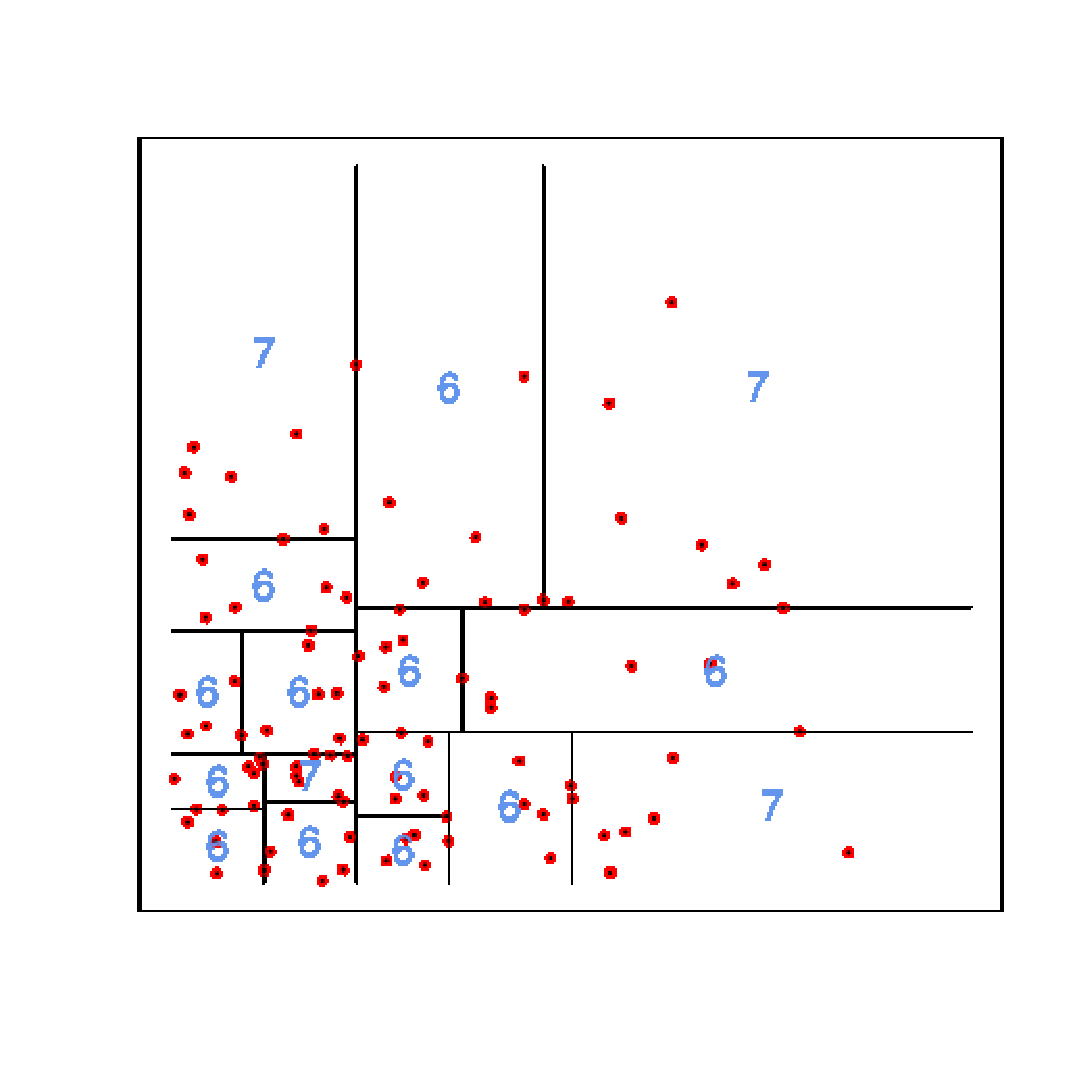
\includegraphics[width=0.3\textwidth]{goodCard.eps}
	}
	\hspace{3pt}%
	\subfloat[][Uniformly distributed]{%
		\label{fig:goodCardUnif}
		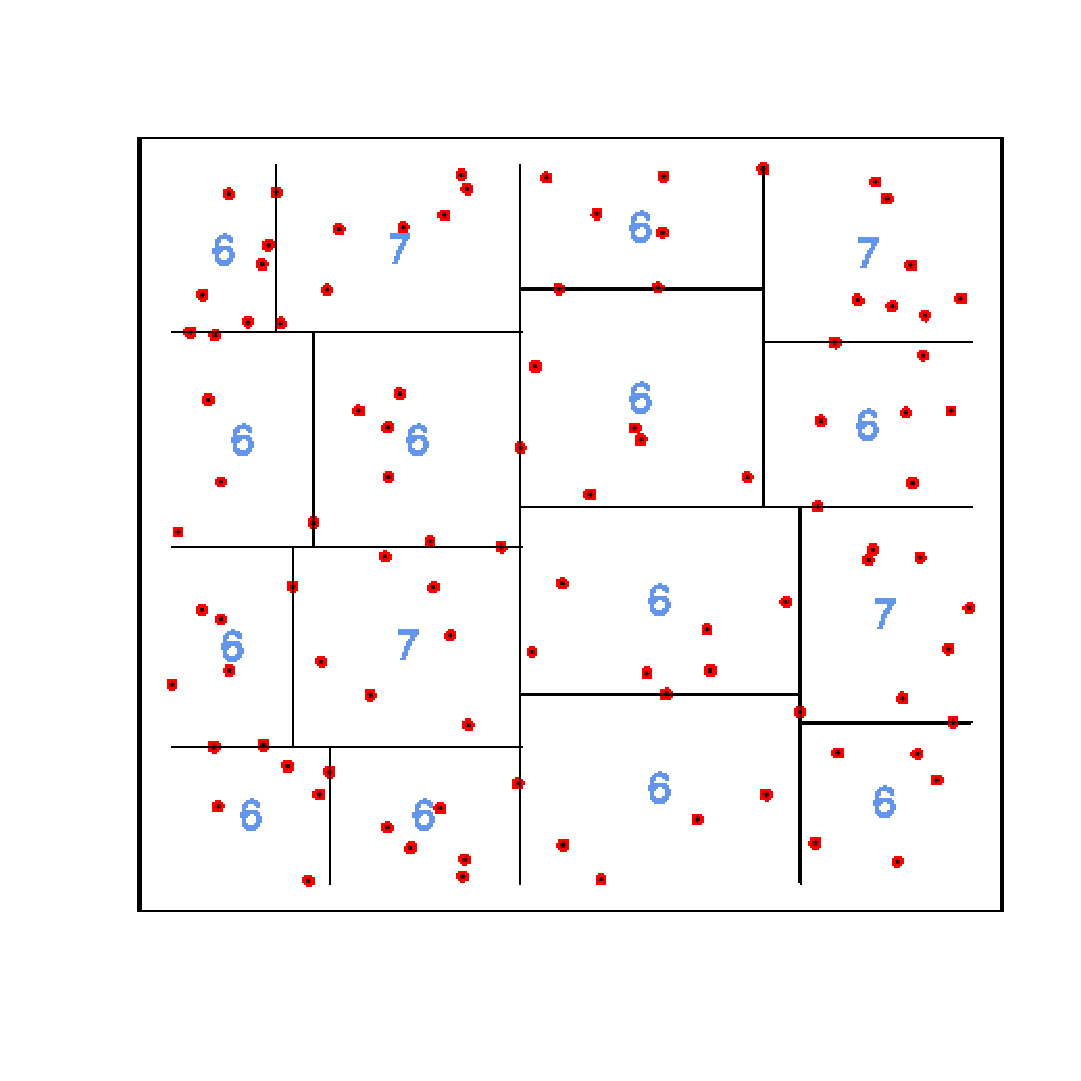
\includegraphics[width=0.3\textwidth]{goodCard2.eps}
	}\\
	\subfloat[][Normally distributed]{
		\label{fig:goodMeanNorm}
		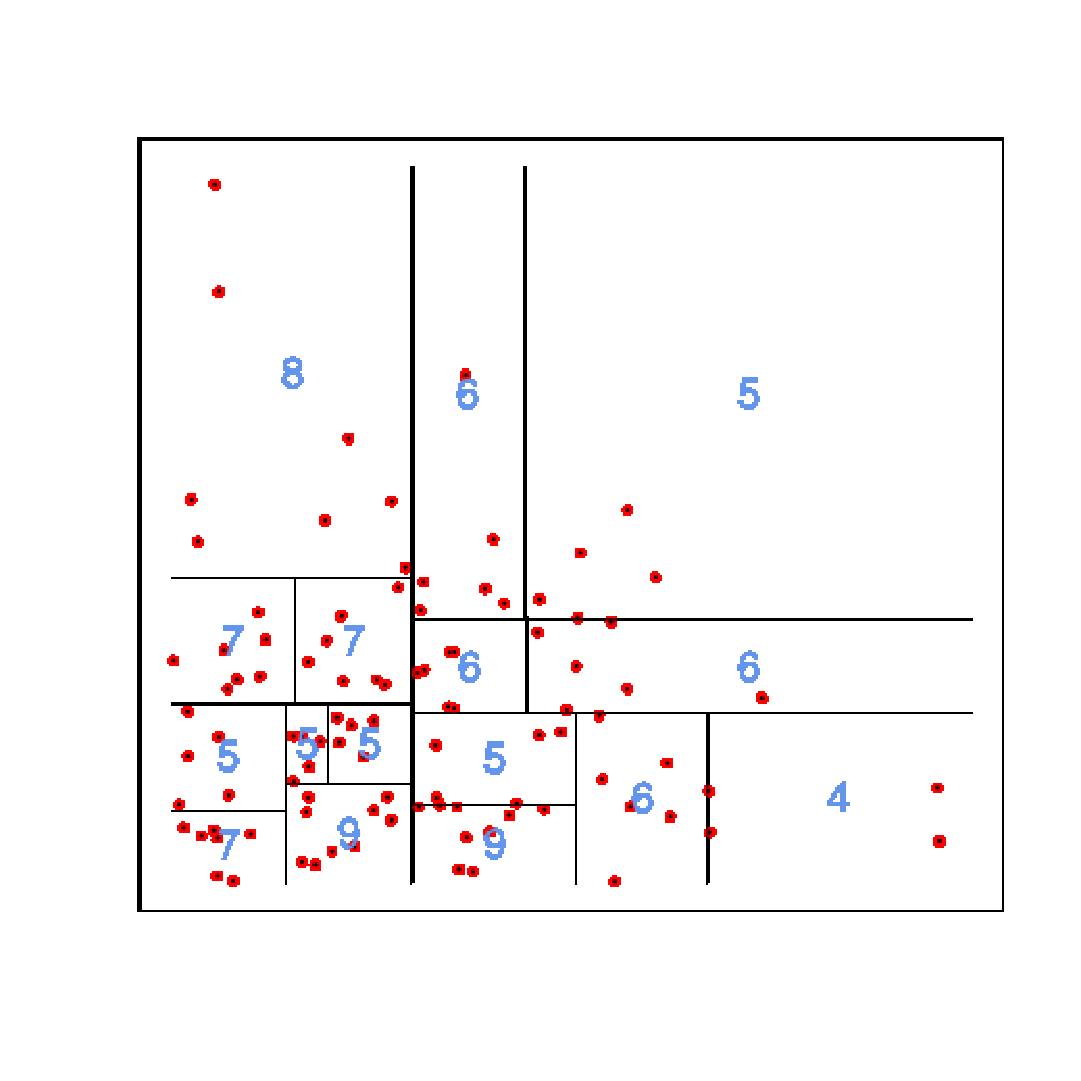
\includegraphics[width=0.3\textwidth]{goodMean.eps}
	}
	\hspace{3pt}%
	\subfloat[][Uniformly distributed]{%
		\label{fig:goodMeanUnif}
		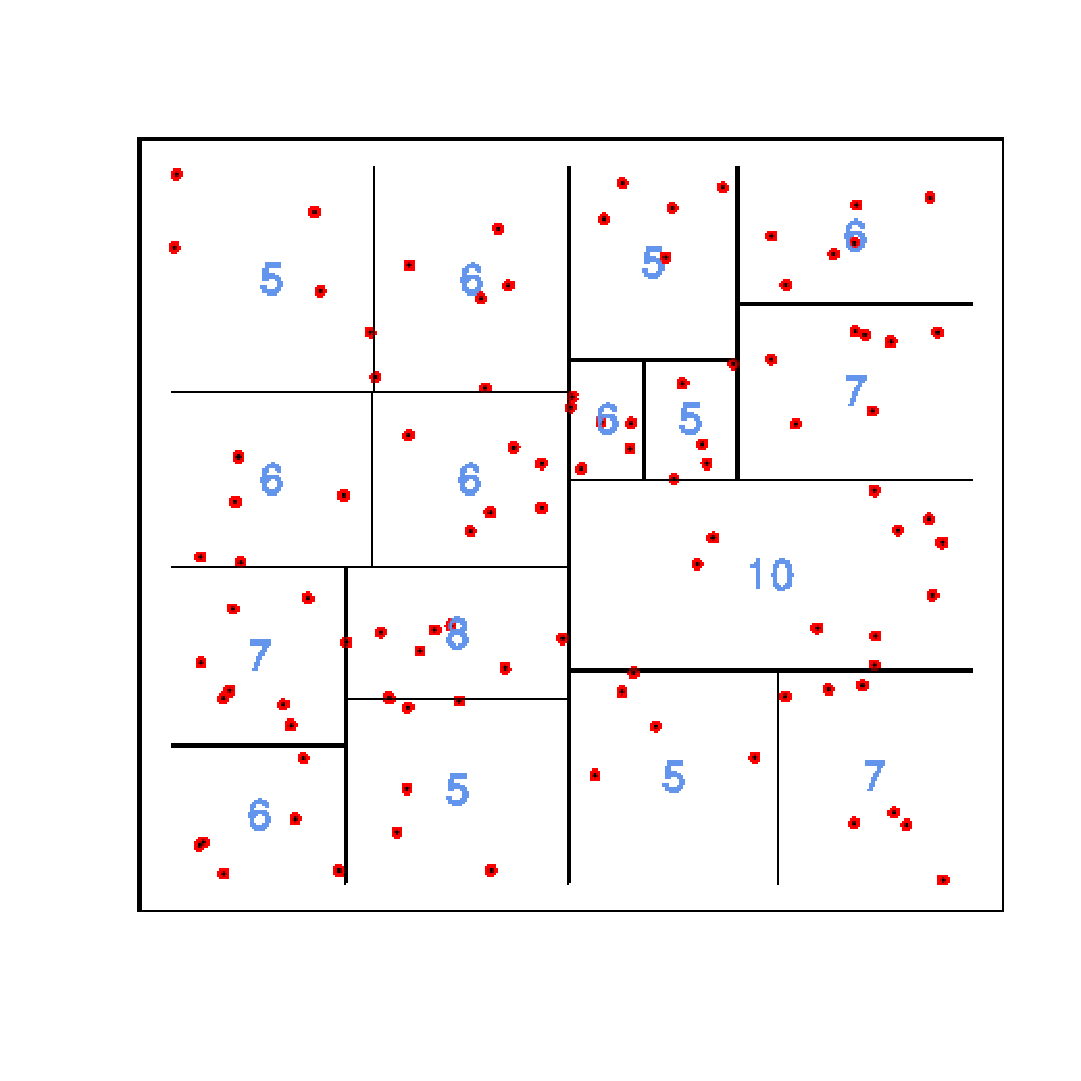
\includegraphics[width=0.3\textwidth]{goodMean2.eps}
	}
	\caption[]{Domain divided in $2^4 = 16$ sub-domains:
		\subref{fig:goodCardNorm} -
		\subref{fig:goodCardUnif} Cardinal;
		\subref{fig:goodMeanNorm} -	
		\subref{fig:goodMeanUnif} Mean.}%
	\label{fig:goodCard}
\end{figure}

%\textcolor{orange}{
%Is easy to see that this strategy guarantees that every built subset has at most two times the elements of some other. Let's take a look to the following example, but first we need to remember that: }
%
%\begin{itemize}
%\item \textcolor{orange}{The point is that every time we choose the most populated set to be divided}
%\item \textcolor{orange}{The current sub-domain is divided in two sub-sub-domains with the same cardinality.}
%\end{itemize} 
%
%\begin{example}
%\textcolor{orange}{
%This example will allow us to intuitively prove the above affirmation.}
%
%\textcolor{orange}{Suppose that there is a sub-domain $A$ in the list with more than two-times the number of element of some other and let's call it $B$. In other words:}
%
%$$\left| A\right| = 2\cdot k\cdot\left| B\right|$$
%$$\text{with } k \in \mathbb{Z}^+$$
%
%\textcolor{orange}{In that case, $B$ was built splitting some other with $\left(2\cdot (k-1)\cdot\left| B\right|\right)$ elements, and it was selected to be divided instead of $A$: \sc{Contradiction!!}}
%\end{example}
%
%\textcolor{orange}{This problem can be avoided forcing the algorithm to generate a quantity of sub-domains power of 2 (see Figure \ref{fig:goodCard}).}

\section{Conclusion}

In this section I present a theoretical and not validated work where I have applied the {\it search space subdivision} approach to solve {\it k-medoids problem} in parallel. I have proposed some different strategies and I have showed graphically some characteristics of them. 